% Short version of the methods note (target: about 5,000 body words).
% The full version is main.tex; both read numbers.tex, refs.bib and figures/ from the same build.
\documentclass[11pt]{article}
\usepackage[margin=1in]{geometry}
\usepackage{amsmath,amssymb,amsthm}
\usepackage{graphicx}
\usepackage{booktabs}
\usepackage{natbib}
\usepackage[hidelinks]{hyperref}
\usepackage{xcolor}
\usepackage{framed}

\newtheorem{proposition}{Proposition}
% Written by make_figures.py; do not edit.
\newcommand{\CaseCentredRawAnchorCosIdx}{161}
\newcommand{\CaseCentredRawAnchorCosPass}{56\%}
\newcommand{\CaseCentredRawAnchorEucIdx}{189}
\newcommand{\CaseCentredRawAnchorEucPass}{55\%}
\newcommand{\CaseCentredRawAnchorInter}{+0.035}
\newcommand{\CaseCentredRawAnchorP}{4e-15}
\newcommand{\CaseCentredRawGatedCosIdx}{138}
\newcommand{\CaseCentredRawGatedCosPass}{61\%}
\newcommand{\CaseCentredRawGatedEucIdx}{160}
\newcommand{\CaseCentredRawGatedEucPass}{58\%}
\newcommand{\CaseCentredRawGatedInter}{+0.015}
\newcommand{\CaseCentredRawGatedP}{0.025}
\newcommand{\CaseCentredRunAnchorCosIdx}{161}
\newcommand{\CaseCentredRunAnchorCosPass}{54\%}
\newcommand{\CaseCentredRunAnchorEucIdx}{189}
\newcommand{\CaseCentredRunAnchorEucPass}{55\%}
\newcommand{\CaseCentredRunAnchorInter}{+0.034}
\newcommand{\CaseCentredRunAnchorP}{5.7e-15}
\newcommand{\CaseCentredRunGatedCosIdx}{143}
\newcommand{\CaseCentredRunGatedCosPass}{58\%}
\newcommand{\CaseCentredRunGatedEucIdx}{160}
\newcommand{\CaseCentredRunGatedEucPass}{58\%}
\newcommand{\CaseCentredRunGatedInter}{+0.013}
\newcommand{\CaseCentredRunGatedP}{0.046}
\newcommand{\CaseCentredTzeroAnchorCosIdx}{167}
\newcommand{\CaseCentredTzeroAnchorCosPass}{34\%}
\newcommand{\CaseCentredTzeroAnchorEucIdx}{189}
\newcommand{\CaseCentredTzeroAnchorEucPass}{55\%}
\newcommand{\CaseCentredTzeroAnchorInter}{+0.032}
\newcommand{\CaseCentredTzeroAnchorP}{4.2e-14}
\newcommand{\CaseCentredTzeroGatedCosIdx}{163}
\newcommand{\CaseCentredTzeroGatedCosPass}{32\%}
\newcommand{\CaseCentredTzeroGatedEucIdx}{160}
\newcommand{\CaseCentredTzeroGatedEucPass}{58\%}
\newcommand{\CaseCentredTzeroGatedInter}{+0.003}
\newcommand{\CaseCentredTzeroGatedP}{0.6}
\newcommand{\CaseUnitRawAnchorCosIdx}{147}
\newcommand{\CaseUnitRawAnchorCosPass}{100\%}
\newcommand{\CaseUnitRawAnchorEucIdx}{189}
\newcommand{\CaseUnitRawAnchorEucPass}{55\%}
\newcommand{\CaseUnitRawAnchorInter}{+0.038}
\newcommand{\CaseUnitRawAnchorP}{8.6e-18}
\newcommand{\CaseUnitRawGatedCosIdx}{124}
\newcommand{\CaseUnitRawGatedCosPass}{100\%}
\newcommand{\CaseUnitRawGatedEucIdx}{160}
\newcommand{\CaseUnitRawGatedEucPass}{58\%}
\newcommand{\CaseUnitRawGatedInter}{+0.018}
\newcommand{\CaseUnitRawGatedP}{0.0097}
\newcommand{\CaseUnitRunAnchorCosIdx}{187}
\newcommand{\CaseUnitRunAnchorCosPass}{53\%}
\newcommand{\CaseUnitRunAnchorEucIdx}{189}
\newcommand{\CaseUnitRunAnchorEucPass}{55\%}
\newcommand{\CaseUnitRunAnchorInter}{+0.020}
\newcommand{\CaseUnitRunAnchorP}{1.7e-08}
\newcommand{\CaseUnitRunGatedCosIdx}{478}
\newcommand{\CaseUnitRunGatedCosPass}{57\%}
\newcommand{\CaseUnitRunGatedEucIdx}{160}
\newcommand{\CaseUnitRunGatedEucPass}{58\%}
\newcommand{\CaseUnitRunGatedInter}{-0.057}
\newcommand{\CaseUnitRunGatedP}{1.2e-12}
\newcommand{\CaseUnitTzeroAnchorCosIdx}{174}
\newcommand{\CaseUnitTzeroAnchorCosPass}{72\%}
\newcommand{\CaseUnitTzeroAnchorEucIdx}{189}
\newcommand{\CaseUnitTzeroAnchorEucPass}{55\%}
\newcommand{\CaseUnitTzeroAnchorInter}{+0.026}
\newcommand{\CaseUnitTzeroAnchorP}{1.9e-11}
\newcommand{\CaseUnitTzeroGatedCosIdx}{363}
\newcommand{\CaseUnitTzeroGatedCosPass}{72\%}
\newcommand{\CaseUnitTzeroGatedEucIdx}{160}
\newcommand{\CaseUnitTzeroGatedEucPass}{58\%}
\newcommand{\CaseUnitTzeroGatedInter}{-0.037}
\newcommand{\CaseUnitTzeroGatedP}{6.3e-07}
\newcommand{\CentredCosMax}{50\%}
\newcommand{\CentredCosMin}{50\%}
\newcommand{\CentredEucEight}{0.5\%}
\newcommand{\CentredEucTwo}{48\%}
\newcommand{\DiagAllCos}{124}
\newcommand{\DiagAllEuc}{162}
\newcommand{\DiagFixCosHi}{78}
\newcommand{\DiagFixCosLo}{77}
\newcommand{\DiagFixEucHi}{134}
\newcommand{\DiagFixEucLo}{124}
\newcommand{\DiagOrigCos}{78}
\newcommand{\DiagOrigEuc}{134}
\newcommand{\DiagTrustCos}{117}
\newcommand{\DiagTrustEuc}{169}
\newcommand{\DriftCos}{33\%}
\newcommand{\DriftEuc}{62\%}
\newcommand{\MatchCentredAng}{0.95}
\newcommand{\MatchCentredCos}{0.42}
\newcommand{\MatchCentredEuc}{1.01}
\newcommand{\MatchUnitAng}{0.36}
\newcommand{\MatchUnitCos}{0.07}
\newcommand{\MatchUnitEuc}{0.51}
\newcommand{\MinCells}{18}
\newcommand{\MinCosAngPassDiff}{0.006}
\newcommand{\MinCosAngVarDiff}{0.00}
\newcommand{\MinRawGroupClose}{42\%}
\newcommand{\MinRawGroupGap}{0.68}
\newcommand{\MinRawGroupGapMax}{7.1}
\newcommand{\MinRawPassGap}{0.19}
\newcommand{\MinRawVarGap}{1.32}
\newcommand{\MinRawVarGapMax}{+2.72}
\newcommand{\MinRawVarGapMin}{-6.49}
\newcommand{\MinRunGroupClose}{83\%}
\newcommand{\MinRunGroupGap}{0.08}
\newcommand{\MinRunGroupGapMax}{3.7}
\newcommand{\MinRunPassGap}{0.01}
\newcommand{\MinRunVarGap}{0.61}
\newcommand{\MinRunVarGapMax}{+2.58}
\newcommand{\MinRunVarGapMin}{+0.02}
\newcommand{\MinTzeroGroupClose}{33\%}
\newcommand{\MinTzeroGroupGap}{0.78}
\newcommand{\MinTzeroGroupGapMax}{4.9}
\newcommand{\MinTzeroPassGap}{0.16}
\newcommand{\MinTzeroVarGap}{1.18}
\newcommand{\MinTzeroVarGapMax}{+3.41}
\newcommand{\MinTzeroVarGapMin}{+0.02}
\newcommand{\UnitFourAng}{32\%}
\newcommand{\UnitFourCos}{94\%}
\newcommand{\UnitFourEuc}{14\%}
\newcommand{\UnitSixteenCos}{99.7\%}
\newcommand{\UnitSixteenEuc}{0.0\%}
   % every number in the text, written by make_figures.py
\newcommand{\ArchiveDOI}{\textbf{[Zenodo DOI to be added]}}

\title{Hidden Choices: How Thresholds, Origins and Tests Manufacture and Hide Effects in Bounded-Confidence Models}
\author{Krishnasai Addala\\ \small Independent researcher}
\date{Short draft of \today}

\begin{document}
\maketitle

\begin{abstract}
Comparing distance measures in multidimensional bounded-confidence models involves choices that are easy to leave unstated.
We follow five of them, each met while auditing our own model.
In an agent-based model of AI governance, a draft finding that geometry reverses the effect of enforcement lag came from reading each geometry against a benchmark; the test that compares the geometries keeps its sign from the draft's model to the audited one (interaction \VCDraftInter\ and \VCRecommendedInter).
The point toward which low trust pulls the perceived policy, which nobody had measured, moved the cosine result across that benchmark and, for one of four defensible targets, removed the difference between geometries.
In a minimal Deffuant model, one shared threshold admits very different shares of opinion pairs under Euclidean, cosine and angular distance; matching the threshold at the start leaves interaction rates apart, and matching it over the run equalises them but not the number of opinion groups, so each matched point answers a different question.
Counting groups with each geometry's own radius made two identical gates look different.
We close with a six-item audit list.
\end{abstract}

\section{Introduction}

Bounded-confidence (BC) models let two agents influence each other only when their opinions are close enough \citep{deffuant2000,hegselmann2002}.
With several opinion dimensions, ``close enough'' needs a distance, and comparing distances has become a modelling question of its own.
Such a comparison involves five choices that can each create an effect or hide one:
\begin{enumerate}
\item \textbf{which test is read}: each condition against a benchmark, or the comparison itself;
\item \textbf{where the origin sits}, for angular gates and for any step that shrinks a quantity toward a point;
\item \textbf{the threshold value} given to each distance measure;
\item \textbf{when coverage is matched}: at the start of a run or over the run;
\item \textbf{how outcomes are counted}: the radius used to group final opinions, and when the run is stopped.
\end{enumerate}
We met every one of them while auditing our own model.
In an unpublished draft we reported that, in an agent-based model of AI governance, geometry \emph{reverses} the effect of enforcement lag on shocks.
The first two choices produced that reading (Section~\ref{sec:case}).
Section~\ref{sec:minimal} then takes the other three in a minimal Deffuant model, and Section~\ref{sec:protocol} collects the lessons into an audit list.
The note is pre-emptive: we do not estimate how often published studies make these choices.
A longer version with every per-cell result, the gate~$\times$~update-step crossing and a fuller literature review is in the repository (Code and data).

\paragraph{Related work.}
\citet{lorenz2008} compared the $L_1$ and $L_\infty$ norms after rescaling the threshold so that their confidence regions had equal volume, and \citet{li2026} note that lowering a topic weight at a fixed bound enlarges the region of agreement as well as changing its shape.
We extend volume matching to \emph{coverage}, the share of actual opinion pairs a gate admits, which also works for angular gates whose regions have no finite volume, and then to matching over the run.
\citet{flache2017} call for systematic comparisons of social-influence models; model docking \citep{axtell1996,wilensky2007} showed that settings that look like implementation details carry substantive assumptions, and \citet{gilbert2018} argue that a policy model's assumptions must be visible to be useful.
The origin audit, coverage and pass-rate matching, and the common ruler are, as far as we know, new; testing the interaction \citep{gelman2006} and using equivalence tests \citep{lakens2017} restate standard advice in this setting.

\section{Background}
\label{sec:background}

A \emph{geometry} is a distance measure, used by the gate, together with its update step.
For opinion vectors $x_i, x_j$ we use Euclidean distance $\lVert x_i - x_j\rVert$, cosine distance $1-\cos\theta_{ij}$ and the angle $\theta_{ij}$ between them.
The gate lets two agents converse when their distance is at most the threshold $\varepsilon$; the listener then moves a fraction $r$ of the way toward the speaker, along a straight line for Euclidean distance and by rotating its opinion, keeping its length, for the two angular geometries.
Because cosine distance is a strictly increasing function of the angle, a cosine gate at $\varepsilon$ and an angular gate at $\arccos(1-\varepsilon)$ admit exactly the same pairs: once matched, the two can differ only through their update steps and how outcomes are measured.

A gate's \emph{coverage} is the share of opinion pairs within its threshold at one moment, and its \emph{pass rate} the share of attempted conversations that pass it during a run.
A comparison can give every geometry Euclidean's threshold number (\emph{shared}), the threshold that gives the same coverage at the start (\emph{start-matched}), or the threshold that gives the same pass rate over the run (\emph{run-matched}).

Euclidean distance and the Euclidean step are unchanged by shifting and rescaling the opinion space; angular gates and steps are not, since they measure direction from the origin.
The same holds for multiplicative shrinkage of a signal (such as a policy scaled by trust), decay toward zero, clipping after a non-equivariant step, zero initial values and ratio outcomes.
If opinions are coded in $[0,1]^d$, all of these refer to the corner where every dimension is at its minimum.

\section{The test and the origin, in a governance model}
\label{sec:case}

\subsection{Model and claim}
PolicySwarm \citep{policyswarm} models how a population's views on AI regulation respond to a policy, to media and to shocks (Appendix~\ref{app:policyswarm}).
Agents hold four-dimensional opinions on a Barab\'asi--Albert network and converse under a bounded-confidence gate.
After an enforcement lag, each agent is pulled toward the policy as it perceives it: $a_i + \tau_i(p + b_i - a_i) + \eta$, where $p$ is the policy, $\tau_i \in [0,1]$ the agent's trust, $b_i$ its ideological bias, $\eta$ noise and $a_i$ the \emph{trust target}, the point a low-trust agent's perceived policy is pulled toward.

The experiment compares paired runs with and without a schedule of shocks, which pull their targets toward the neutral centre and so lower the final variance of opinions.
The \emph{relative shock effect} is that change in variance divided by the variance of the run without shocks, and it is negative.
Runs are made at enforcement lags of 0, 20 and 40 ticks.
For each geometry the \emph{lag index} is the mean relative shock effect at lag 40 as a percentage of its mean at lag 0, by size.
The \emph{interaction} is cosine's change from lag 0 to lag 40 minus Euclidean's, paired by seed; with negative effects, a positive interaction means lag enlarges the effect less under cosine, so that cosine \emph{attenuates} the lag effect.
The index is a proportional change within one geometry, and the interaction compares the two on one scale; since cosine's lag-0 effect is about half Euclidean's, the two can disagree, and we rest claims about geometry on the interaction.

The draft reported, on the absolute shock effect, an index of about 130 under Euclidean distance and about 75 under cosine distance, and called it a reversal.
Read as policy advice, whether delays in enforcement make a population more or less fragile after shocks would have hinged on an untested modelling choice.
An internal audit found the problem before any external use (pre-audit engine: commit \texttt{50a42e5}).

\subsection{Design}
We ran the audited engine with the draft's choices restored as switches: the gate measured from the cube's corner or its centre, the threshold shared or matched, the policy pull applied only after a conversation that passes the gate (as in the draft) or every tick, and four trust targets (the corner, the centre, the population's mean starting opinion, and the agent's own opinion).
We also ran the draft's own engine with the audit's other fixes undone in turn, and a \emph{level-shift} control that moves every agent's perceived policy by the corner's average shift, $-(1-\bar\tau)$, separating a shift in the mean from one that differs between trusting and distrustful agents.
The \emph{recommended} design uses a centred gate, a run-matched threshold and a pull applied every tick, which removes both of the draft's couplings.
Every cell crosses Euclidean and cosine with the three lags over 100 paired seeds.
We report each lag index with a paired bootstrap 95\% interval and the interaction with a 95\% $t$ interval, and call an interaction equivalent to zero when its 90\% interval lies within $\pm\VInterMargin$; we set this margin after an earlier version had reported the result it is used on, so that test confirms a result already known.

\subsection{Results}

\begin{figure}[t]
\centering
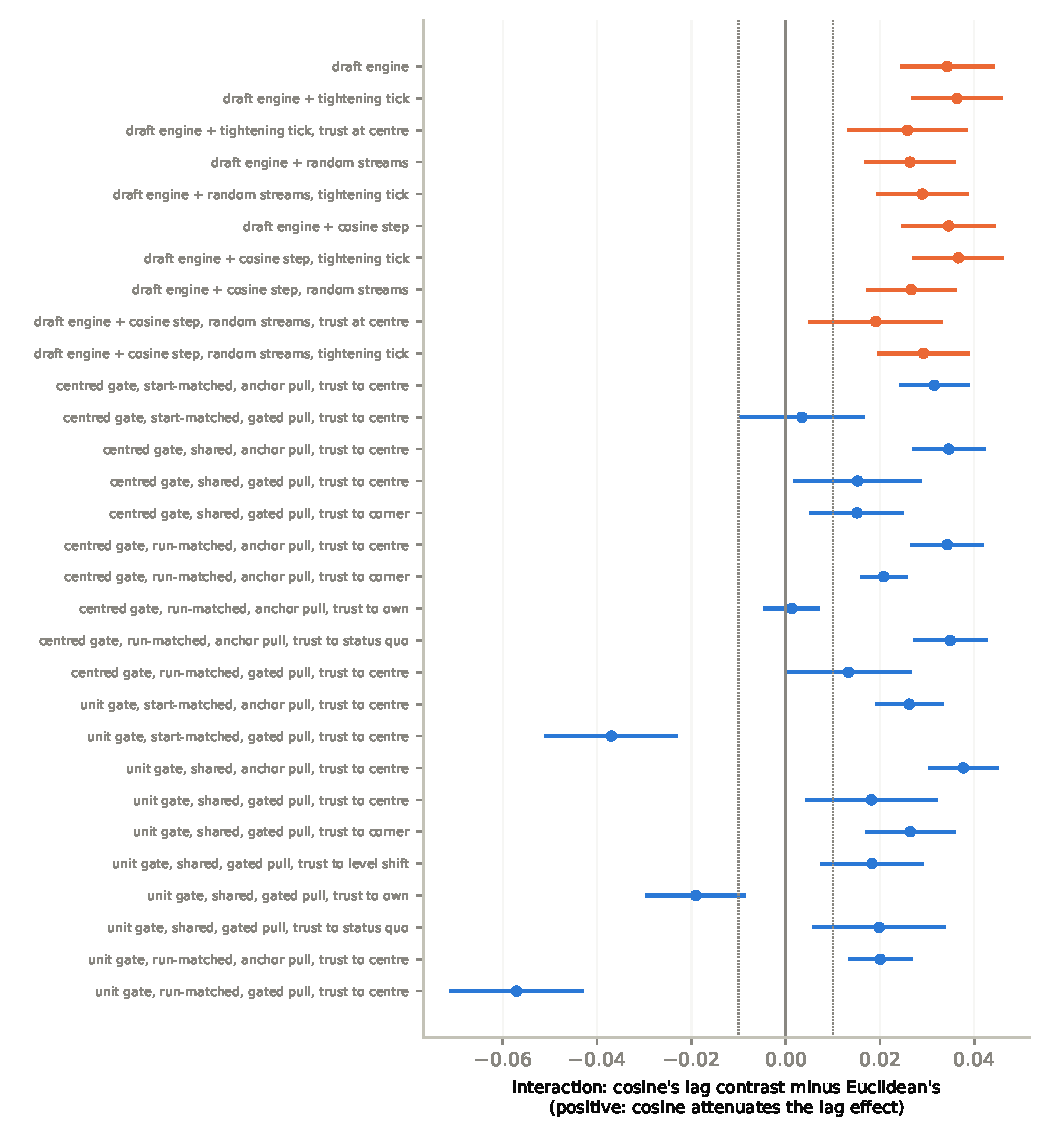
\includegraphics[width=\linewidth]{figures/fig4_interaction_all_cells.pdf}
\caption{The lag $\times$ geometry interaction in every configuration (cosine's lag contrast minus Euclidean's; positive: cosine attenuates the lag effect), with 95\% $t$ intervals over 100 paired seeds; dotted lines mark the equivalence margin. Orange: the draft's engine, alone or with the audit's changes named in the label. Blue: the audited engine, by gate space, threshold rule, policy pull and trust target.}
\label{fig:interaction}
\end{figure}

\paragraph{The test.}
Across all \VCaseCells\ configurations the interaction is positive in \VCasePositive, negative in \VCaseNegative\ and not significantly different from zero in \VCaseNull\ (Figure~\ref{fig:interaction}).
In the draft's own engine and settings it is \VCDraftInter\ \VCDraftCI, the same direction as in the audited model.
What looked like a reversal was cosine's index falling below 100 (\VCDraftCosAbsIdx\ on the absolute effect the draft used, against \VCDraftEucAbsIdx\ for Euclidean) while the comparison between geometries kept its sign.
Reading each geometry against 100 asks whether each effect grows with lag; the claim was about the difference between geometries, and only the interaction tests that \citep{gelman2006}.
Two of the negative cells come from an uncentred gate with a matched threshold and the gated pull, where the matched cosine thresholds are tiny because all opinions point into one orthant; the third is a trust target (below).

\paragraph{Which comparison isolates the threshold.}
The centred cells hold the gate fixed and vary only the threshold rule.
With the pull applied every tick, the interaction barely moves across the shared, start-matched and run-matched rules (\VFCentredRawAnchorInter, \VFCentredMatchedAnchorInter, \VFCentredRunAnchorInter).
In the unit cube the same change of threshold moves it from \VFUnitRawAnchorInter\ to \VFUnitRunAnchorInter, and with the gated pull from \VFUnitRawGatedInter\ to \VFUnitRunGatedInter: the threshold matters here mainly through the uncentred gate.

\paragraph{The origin.}
With trust shrinking toward the corner and angles measured from the corner, as in the draft, the audited engine gives Euclidean \VTUnitRawCornerEucIdx\ and cosine \VTUnitRawCornerCosIdx, matching the draft's engine (\VCDraftFixedEucIdx\ and \VCDraftFixedCosIdx).
Shrinking toward the centre lifts cosine to \VTUnitRawCentreCosIdx; measuring the gate from the centre lifts it to \VTCentredRawCornerCosIdx.
In this setting Euclidean's index barely moves with the trust target, and the level shift takes cosine only to \VTUnitRawLevelShiftCosIdx: most of the corner's effect comes from shifting distrustful agents further than trusting ones, which an angle measured from the corner registers.
The interaction stays positive throughout (\VTUnitRawCornerInter, \VTUnitRawCentreInter, \VTUnitRawLevelShiftInter): the origin moved cosine's index across 100 but left the sign of the comparison unchanged.

\begin{table}[t]
\centering\small
\caption{Trust targets in the recommended design: lag index per geometry (95\% CI), relative shock effect at lags 0 and 40 for Euclidean (E) and cosine (C), and the paired interaction; $^{=}$ marks equivalence to zero.}
\label{tab:anchors}
\begin{tabular}{lrrrr}
\toprule
trust target & Euclidean index & cosine index & lag-0 effect (E / C) & interaction [95\% CI] \\
\midrule
centre & 146 [138, 154] & 134 [129, 139] & -0.119 / -0.060 & +0.034 [+0.027, +0.042] \\
corner & 121 [116, 125] & 106 [103, 109] & -0.121 / -0.071 & +0.021 [+0.016, +0.025] \\
own & 113 [109, 116] & 128 [125, 132] & -0.182 / -0.077 & +0.001 [-0.004, +0.007]$^{=}$ \\
status quo & 147 [138, 156] & 134 [129, 140] & -0.119 / -0.059 & +0.035 [+0.027, +0.042] \\
\bottomrule
\end{tabular}

\end{table}

\paragraph{The trust target is an assumption.}
Trust has to shrink the perceived policy toward something, and the four targets give different answers (Table~\ref{tab:anchors}).
The status quo behaves like the centre, as it must when starting opinions are uniform.
Shrinking toward the corner leaves lag little effect under cosine (\VTCentredRunCornerCosIdx).
Shrinking toward the agent's own opinion makes the interaction equivalent to zero (\VTCentredRunOwnInter, 90\% interval \VTCentredRunOwnCINinety), and in the draft's setting the same target makes it negative (\VTUnitRawOwnInter).
Across the four targets, Euclidean's lag index alone runs from \VTargetEucMin\ to \VTargetEucMax.
The right target depends on how distrust distorts a policy signal, which the model cannot decide, so a study using such a model should state the target and vary it.

\paragraph{The remaining effect.}
In the recommended design with trust shrinking toward the centre, lag enlarges the shock effect under both geometries and less under cosine (indices \VCRecommendedEucIdx\ and \VCRecommendedCosIdx; interaction \VCRecommendedInter\ \VCRecommendedCI).
We would report this result, with the condition the target sweep attaches to it.

\section{The other three choices, in a minimal model}
\label{sec:minimal}

\subsection{Design}
A minimal Deffuant model (Appendix~\ref{app:odd}) has 500 agents on an Erd\H{o}s--R\'enyi graph, random matchings each round and $\mu = 0.3$.
The factorial crosses the opinion space (unit or centred cube), the dimension ($d \in \{2,4,8\}$) and a reference coverage ($5\%$, $15\%$, $30\%$): 18 cells, 100 paired seeds each.
Euclidean distance runs at the threshold giving the reference coverage at the start; cosine and angular distance run under the shared, start-matched and run-matched rules, and under an \emph{early-matched} rule that matches the pass rate over the first 100 rounds only.
Matched thresholds were found by bisection on 50 separate pilot seeds and checked on the evaluation seeds.
The primary outcome is the number of opinion groups holding at least 1\% of agents after 2{,}000 rounds, counted with one ruler for every geometry.
We call a gap equivalent to zero when its 90\% interval lies within $\pm0.02$ for the pass rate or $\pm0.25$ on the $\log_2$ scale \citep{lakens2017}.
Cosine and angular are reported separately, but they agree closely, so the text gives cosine and Table~\ref{tab:headline} both.

\subsection{Results}

\paragraph{The threshold value.}
One shared number admits very different shares of pairs: in the unit cube at $\varepsilon = 0.5$, a cosine gate admits \UnitFourCos\ of pairs in four dimensions against \UnitFourEuc\ for Euclidean distance (Table~\ref{tab:coverage}).
As the dimension grows, distances concentrate \citep{aggarwal2001}:

\begin{proposition}[Coverage at a fixed threshold]
For independent uniform opinions, as $d \to \infty$, $\lVert x_i - x_j\rVert/\sqrt d$ converges to $1/\sqrt6$ in $[0,1]^d$ and to $\sqrt{2/3}$ in $[-1,1]^d$; $\cos\theta_{ij}$ converges to $3/4$ in $[0,1]^d$ and to $0$ in $[-1,1]^d$.
Hence at a fixed threshold, cosine and angular coverage tend to 0 or 1 according to which side of these limits the threshold falls, and Euclidean coverage tends to 0 unless the threshold grows like $\sqrt d$.
\end{proposition}
\noindent Each limit follows from the law of large numbers applied to the coordinate-wise sums; a threshold exactly at an angular limit, such as cosine at $\varepsilon = 1$ in the centred cube, admits half of all pairs in every dimension.
In the minimal model a shared threshold leaves the pass rate apart by a median of \VRawPassGapCos\ (cosine), equivalent to Euclidean's in no cell.

\begin{table}[t]
\centering\small
\begin{tabular}{llrrrr}
\toprule
space & $\varepsilon$ & $d$ & Euclidean & cosine & angular \\
\midrule
unit & 0.5 & 2 & 48\% & 92\% & 58\% \\
unit & 0.5 & 4 & 14\% & 94\% & 32\% \\
unit & 0.5 & 8 & 1\% & 98\% & 15\% \\
unit & 0.5 & 16 & 0\% & 100\% & 4\% \\
centred & 1 & 2 & 48\% & 50\% & 32\% \\
centred & 1 & 4 & 14\% & 50\% & 17\% \\
centred & 1 & 8 & 1\% & 50\% & 7\% \\
centred & 1 & 16 & 0\% & 50\% & 1\% \\
\bottomrule
\end{tabular}

\caption{Share of uniformly drawn pairs admitted at one shared $\varepsilon$, by opinion space and dimension.}
\label{tab:coverage}
\end{table}

\begin{figure}[t]
\centering
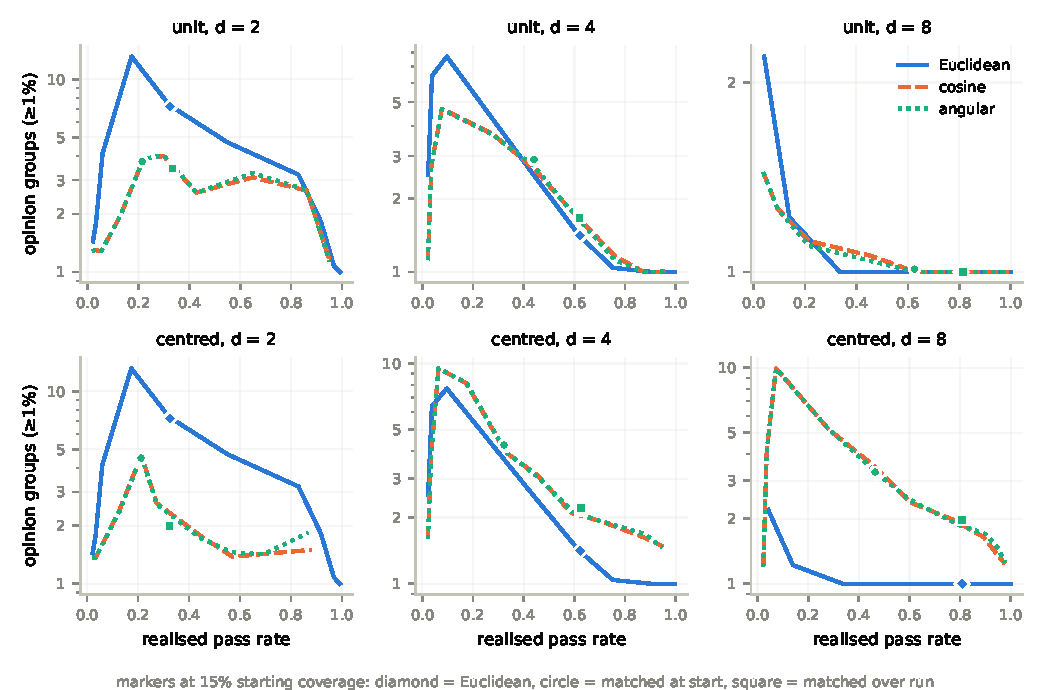
\includegraphics[width=\linewidth]{figures/fig2_response_curves.pdf}
\caption{Number of opinion groups (at least 1\% of agents, common ruler) against the pass rate as the threshold varies over ten values giving starting coverage from 2\% to 60\%; each point is the mean of 50 seeds with a band of $\pm1.96$ standard errors. Markers: the factorial's runs at 15\% starting coverage under each rule. Log scale on the vertical axis.}
\label{fig:curves}
\end{figure}

\begin{table}[t]
\centering\small
\caption{Headline results of the minimal model after 2{,}000 rounds: median absolute gap to Euclidean and the number of the 18 cells equivalent to zero, for cosine and angular. Pass-rate gaps are differences; group gaps are $\log_2$ ratios.}
\label{tab:headline}
\begin{tabular}{llrrrr}
\toprule
 & & \multicolumn{2}{c}{cosine} & \multicolumn{2}{c}{angular} \\
rule & outcome & gap & equiv. & gap & equiv. \\
\midrule
shared & pass rate & \VRawPassGapCos & \VRawPassEquivCos & \VRawPassGapAng & \VRawPassEquivAng \\
 & groups & \VRawGroupGapCos & \VRawGroupEquivCos & \VRawGroupGapAng & \VRawGroupEquivAng \\
start-matched & pass rate & \VTzeroPassGapCos & \VTzeroPassEquivCos & \VTzeroPassGapAng & \VTzeroPassEquivAng \\
 & groups & \VTzeroGroupGapCos & \VTzeroGroupEquivCos & \VTzeroGroupGapAng & \VTzeroGroupEquivAng \\
run-matched & pass rate & \VRunPassGapCos & \VRunPassEquivCos & \VRunPassGapAng & \VRunPassEquivAng \\
 & groups & \VRunGroupGapCos & \VRunGroupEquivCos & \VRunGroupGapAng & \VRunGroupEquivAng \\
early-matched & pass rate & \VEarlyPassGapCos & \VEarlyPassEquivCos & \VEarlyPassGapAng & \VEarlyPassEquivAng \\
 & groups & \VEarlyGroupGapCos & \VEarlyGroupEquivCos & \VEarlyGroupGapAng & \VEarlyGroupEquivAng \\
\bottomrule
\end{tabular}
\end{table}

\paragraph{When coverage is matched.}
Start-matching leaves the pass rate apart by a median of \VTzeroPassGapCos: coverage drifts as opinions converge, faster under Euclidean distance than under the angular geometries, whose steps rotate an opinion without shortening it.
Run-matching equalises the pass rate (equivalent in \VRunPassEquivCos\ of \VCellsPerGeom\ cells) but not the number of groups (\VRunGroupEquivCos\ of \VCellsPerGeom; median gap \VRunGroupGapCos\ on the $\log_2$ scale); early-matching brings the pass rates much closer than start-matching but leaves the group counts as far apart as run-matching does (Table~\ref{tab:headline}).
At equal pass rates the geometries' response curves do not coincide (Figure~\ref{fig:curves}), so the gap depends on where on the curves one compares them.
Matching is therefore a choice of estimand: a start- or early-matched comparison includes a geometry's effect on how often agents interact, and a run-matched one excludes it.
Our first draft reported that run-matching removed the gap because it counted the effective number of groups, an outcome that, once groups have formed, the pass rate nearly fixes.

\paragraph{The gate or the update step?}
Run-matched, the angular geometries still leave final opinions more spread out than Euclidean distance does (median variance gap \VRunVarGapCos\ on the $\log_2$ scale, positive in every cell).
Crossing the gate with the update step shows where that comes from.
With start-matched gates, a Euclidean gate with the cosine step raises the variance by \VXEucCosVar, most of the \VXCosCosVar\ of the pure cosine pairing, while a cosine gate with the Euclidean step raises it by only \VXCosEucVar; with run-matched cosine gates the cosine gate with the Euclidean step even lowers it (\VXRCosEucVar).
The spread of opinion directions follows the gate rather than the step when gates are start-matched (\VXCosEucDisp\ against \VXEucCosDisp), and the gate and step together when they are run-matched.
So the overall spread is mostly the update step's doing, and a comparison that changes the gate and the step at once cannot tell the two apart.

\paragraph{The ruler and the stopping time.}
Our first draft also grouped final opinions within a fraction of each run's own $\varepsilon$.
Start-matched cosine and angular gates admit exactly the same pairs, yet under that rule their group counts are equivalent in only \VCosAngOwnEquiv\ of \VCosAngCells\ cells; with one common ruler they are equivalent in all \VCosAngCommonEquiv, so the apparent difference came from the ruler.
After 500 rounds \VUnsettledFive\ of Euclidean runs are still changing, and after 4{,}000 \VUnsettledFour, but the group gaps barely move over that range (start-matched: \VHorTzeroFive\ to \VHorTzeroFour), so the remaining difference is not a transient; only reporting the stopping time and checking a longer run shows that.

\section{Why this matters}
\label{sec:relevance}

For anyone comparing distance measures, each of the five choices can produce or remove a difference on its own.
In our two models a shared threshold changed the pass rate by a median of \VRawPassGapAng\ to \VRawPassGapCos\ of attempted conversations, a geometry-specific ruler left two identical gates in agreement in only \VCosAngOwnEquiv\ of \VCosAngCells\ cells, and a test read against a benchmark turned an attenuation into a reported reversal.
All three arose without a coding error, and a results table shows none of them unless the choice is reported.

For models used to inform policy, the case study shows a policy-relevant conclusion resting on choices its readers could not see.
Whether enforcement delays make a population more or less fragile after shocks depended on the test read, on where the opinion space put its origin, and on a trust target that no one had measured.
\citet{gilbert2018} argue that a policy model is useful only when its assumptions are visible, and any trust or credibility parameter that shrinks or scales a signal carries an origin with it.

The choices are not specific to distance measures.
Any comparison of model variants that share a free parameter on different scales, shrink a quantity toward a point, or count outcomes with a variant-specific rule meets the same problems, which is the docking problem \citep{axtell1996,wilensky2007} in a narrower form.
We have not measured how often published comparisons make these choices; the audit list below gives a way to check.

\section{An audit list}
\label{sec:protocol}

\begin{framed}
\noindent\textbf{Before reporting that a distance measure changes a result}
\begin{enumerate}
\item \textbf{Test the comparison.} A claim that a geometry changes an effect is an interaction; test it directly \citep{gelman2006}, and support ``no difference'' with an equivalence test \citep{lakens2017}.
\item \textbf{Audit the origin.} Recode the opinion space by a shift and rescale and rerun a few seeds; any outcome that changes depends on the origin. Centre the space at a meaningful neutral point or say why not, and treat every shrinkage or decay target as an explicit, varied assumption.
\item \textbf{Do not rely on a shared threshold value.} If one is used, show that the pass rates match.
\item \textbf{Report the response to $\varepsilon$, not one matched point.} Start-, early- and run-matched points answer different questions; name the one you report, and check calibrated thresholds on separate seeds.
\item \textbf{Check for monotone equivalence.} Distance measures related by a strictly increasing function are one gate once matched.
\item \textbf{Report the ruler and the stopping time.} Count groups with one rule for every geometry, report how many runs have not settled, and check a longer run.
\end{enumerate}
\end{framed}
\noindent Applying the list costs a fraction of the comparison itself: a few reruns or a recount of saved states, about ten thresholds per geometry for the response curves, and one bisection per cell for run-matching.

\section{Limitations}
Opinions start uniform and independent, and we study pairwise Deffuant updates only, without varying $\mu$, the population size or the network.
Runs stop at 4{,}000 rounds, when \VUnsettledFourAll\ of runs have not settled.
The case study rests on one model whose trust mechanism is specific to it, while the general point (multiplicative steps inherit the meaning of the origin) is not.
The five choices are not the only hidden ones: the network, the update order and the population size are choices of the same kind.

\section*{Code and data}
PolicySwarm, the minimal model and every script are archived at \ArchiveDOI\ and developed at \url{https://github.com/D0nu-t/policy-swarm}, together with the longer version of this note and its per-cell results.
\texttt{make\_figures.py} rebuilds every figure, table and number in both versions from the saved results; no number in the text is typed by hand.

\bibliographystyle{apalike}
\bibliography{refs}

\appendix
\section{The minimal model}
\label{app:odd}
Agents hold opinions in $[0,1]^d$ or $[-1,1]^d$ on a fixed Erd\H{o}s--R\'enyi graph with 500 nodes and mean degree 10. Each round draws a random matching of edges, evaluates the gate for every matched pair, and moves both agents of every pair that passes by $\mu = 0.3$ toward each other, then clips to the cube. Initial opinions are independent and uniform; the graph and initial opinions come from one random stream and the matchings from another, so runs that share a seed differ only in the gate, the update step and $\varepsilon$. Outcomes are recorded after 500, 1{,}000, 2{,}000 and 4{,}000 rounds.

\section{PolicySwarm as used in Section~\ref{sec:case}}
\label{app:policyswarm}
120 agents on a Barab\'asi--Albert network ($m=3$) hold opinions in $[-1,1]^4$, an ideology in $[-1,1]$, a fixed trust drawn from Beta(2,\,2) and an influence weight proportional to their degree. Each of 60 ticks applies, in order: a policy tightening at tick 30; scheduled shocks, which move a hub group or ten random agents toward the neutral centre; a media pull scaled by ideology and trust; 150 conversation attempts under the gate, with half blocked by the deployment cap and violators' influence halved after the enforcement lag; the policy pull; and, after the lag, the pull toward the perceived policy defined in Section~\ref{sec:case}, with noise of standard deviation 0.06. The Euclidean threshold is $\varepsilon = 1.0$ in centred coordinates. Paired runs with and without shocks share every other random stream. The longer version lists every parameter and threshold.

\end{document}
